\chapter{Game Design}

Before we start implementing the game, we should design its individual parts.
We need to decide which mechanics will be in the game and how will the player interact with them.
The game needs to react to the player's actions and communicate the information the player should know.
This all depends on what exactly are we trying to achieve.
Thus, we should set some design goals.

\section{Design goals}

We aim to make the game's mechanics clear, and controls intuitive and responsive.
This is a necessity for every game because without this, the players can't even properly play the game you want them to play.
We won't make a subsection specifically for this goal, but it will inform many of our decisions throughout the design.

The following are the goals specific for our game.
We will look at other games for inspiration how these goals could be reached.
The prototype won't achieve any of them well, but they still inform the design of the mechanics we will implement.

\begin{enumerate}
    \item \nameref{sec:goal-depth-battle}
    \item \nameref{sec:goal-depth-run}
    \item \nameref{sec:goal-various-builds}
    \item \nameref{sec:goal-force-exploration}
    \item \nameref{sec:goal-challenge}
\end{enumerate}

\subsection{Strategic Depth in Every Battle} \label{sec:goal-depth-battle}

The player should make meaningful strategic decisions throughout every battle.
Each battle should be different enough to require the player to adapt to the current situation.
This is where the action will happen, but we want the player to make tactical decisions, not test their reflexes.
With this constraint, battles would be boring if every one played out the same.

In \emph{Plants vs.\ Zombies}, the player wants to plant \emph{Sunflowers} or other \emph{sun}-producing plants.
The more they build their economy, the more plants they can afford in the future.
However, these plants can't kill zombies, so the goal is to spend the bare minimum on defense.
This is a hard problem to solve, since when and where zombies will appear is not completely predictable.
What makes this even more complicated are cheap single-use plants like the \emph{Potato Mine}.
It costs only 25\,\emph{sun} and can kill almost any zombie, where, for example, a \emph{Peashooter} costs 100\,\emph{sun}, but is permanent and able to kill tens of zombies over the course of a level.
This means the player always has to consider if it's better to place a plant that's the best now or a plant that will be the best in the future.

\begin{center}
    \captionsetup{type=figure}
    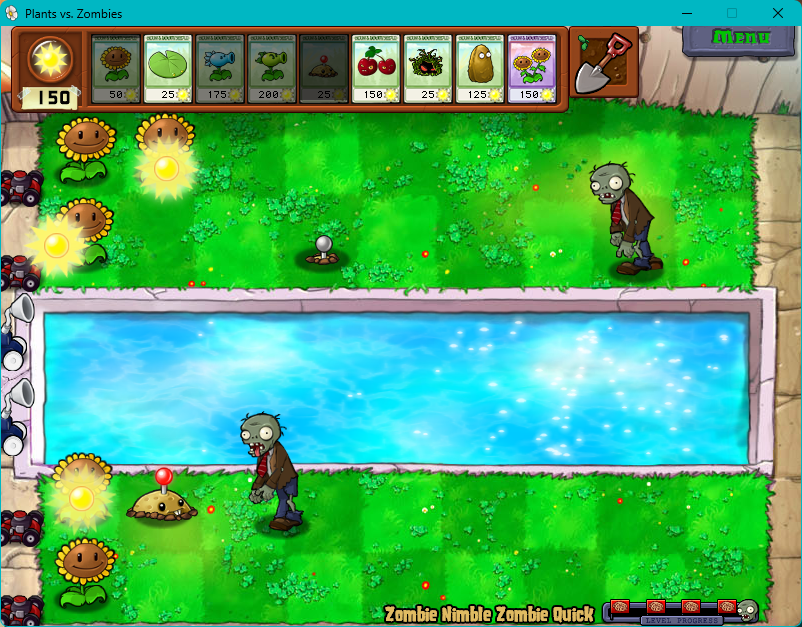
\includegraphics[width=0.8\textwidth]{img/Plants-vs-Zombies-Mines.png}
    \caption{\emph{Sunflowers} and \emph{Potato Mines} in \emph{Plants vs.\ Zombies}. \emph{Sunflowers} are necessary to fuel your economy, while \emph{Potato Mines} are a cheap way to deal with the first few zombies.}
    \label{fig:pvz-mines}
\end{center}

In \emph{Slay the Spire}, the player has to make a similar kind of decision, but even more often.
Almost every enemy grows stronger over time, or makes the player character weaker as they fight.
This means that the player always has to consider when it's the best to defend and when it's better to attack.
The player can choose to not block some damage now in order to kill the enemy sooner and prevent bigger attacks in the future.
The player also has to plan several turns in advance because many cards have longer lasting effects.
\enquote{Is it better to play a card that makes me stronger in the future or a card that helps me now?}

Every fight is different because every enemy has distinctive behavior.
Some enemies get much more powerful over time, so it is important to kill them quickly.
Others punish the player for attacking them, so the player needs to kill them with precision.
Fights also vary a lot because the player draws their cards in a different order every time.
All this means that the player has something to think about every turn.

Our game will also have economic buildings and instant abilities, so the player has to balance economy and short-term versus long-term defense.
The player will have to survive some number of waves, but they will be able to spend extra materials to mine fuel faster and end the battle sooner.
This is similar to being more offensive in \emph{Slay the Spire}, since the waves of attackers should get stronger at a faster pace than the player's defense.
Each battle will require a different approach, since the waves will be composed of a different set of attackers every time.
We can also vary the nature of a battle by changing up the terrain and making attacker paths different lengths or more numerous.
This might seem like too much, but we want to playtest all these options and possibly cut those, which don't work well.

\subsection{Strategic Depth in Every Run} \label{sec:goal-depth-run}

The player should make meaningful strategic decisions throughout every run and there should be no clear path to victory.

In \emph{Slay the Spire}, the player needs to improve many aspects of their deck in tandem.
They need to have great defensive cards, cards that can deal with enemies that have a lot of health, cards that can attack multiple enemies at once and more.
The player should also care about the average cost of the cards in their deck.
It is bad when the player wants to both defend and attack on a given turn, but they've drawn only an expensive attack and an expensive defensive card.
It is also suboptimal when the player plays out all the cards they've drawn, but they have leftover energy they didn't spend.
Balancing these aspects of the deck leads to some difficult decisions when picking cards to add.
For example, should the player pick a good defensive card because they are lacking in defense, or should they pick an attack that's just very strong.

We want to balance the battles in a way, which requires the player to have strong blueprints with various qualities.
The players should need good economic buildings, fuel-producing buildings, abilities and towers good at dealing with various kinds of attackers.
They should also have some cheaper towers to build in the first few waves and more expensive towers to build once they produce a lot of material.

In \emph{Slay the Spire}, the player come across an interesting trade-off between short-term and long-term power, even in building their deck.
The player wants cards which will have a great potential to be strong in the future, having great synergy with other cards.
But these cards aren't strong right now and the player needs to survive the next few fights, making them choose cards that are useful immediately, but might not be as powerful later in the run.
As an example we can look at \emph{Iron Wave} and \emph{Double Tap}.

\begin{center}
    \captionsetup{type=figure}
    \begin{minipage}{.25\textwidth}
        \centering
        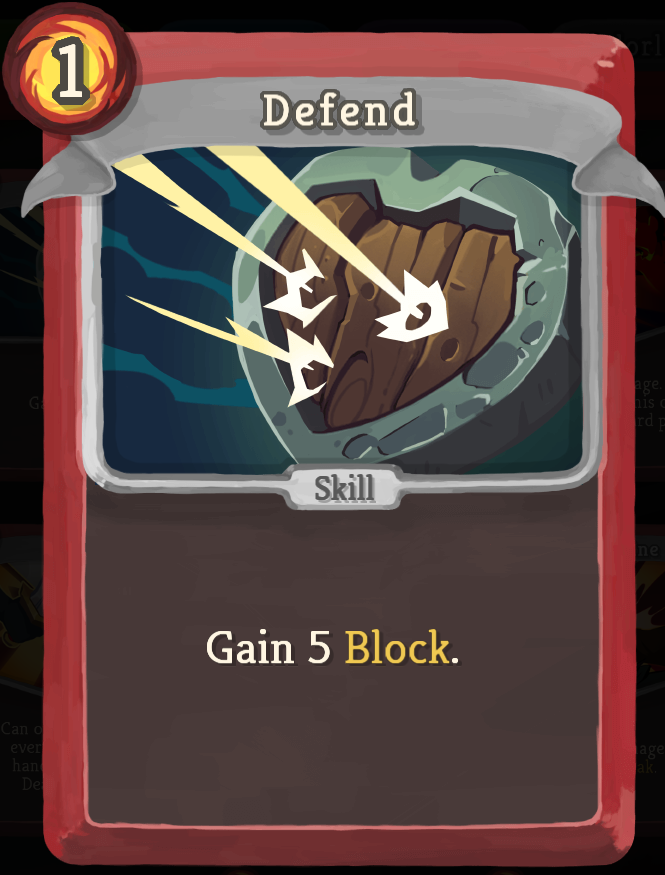
\includegraphics[width=0.95\textwidth]{img/Slay-the-Spire-Defend.png}
        \label{fig:sts-defend}
    \end{minipage}%
    \begin{minipage}{.25\textwidth}
        \centering
        \captionsetup{justification=centering}
        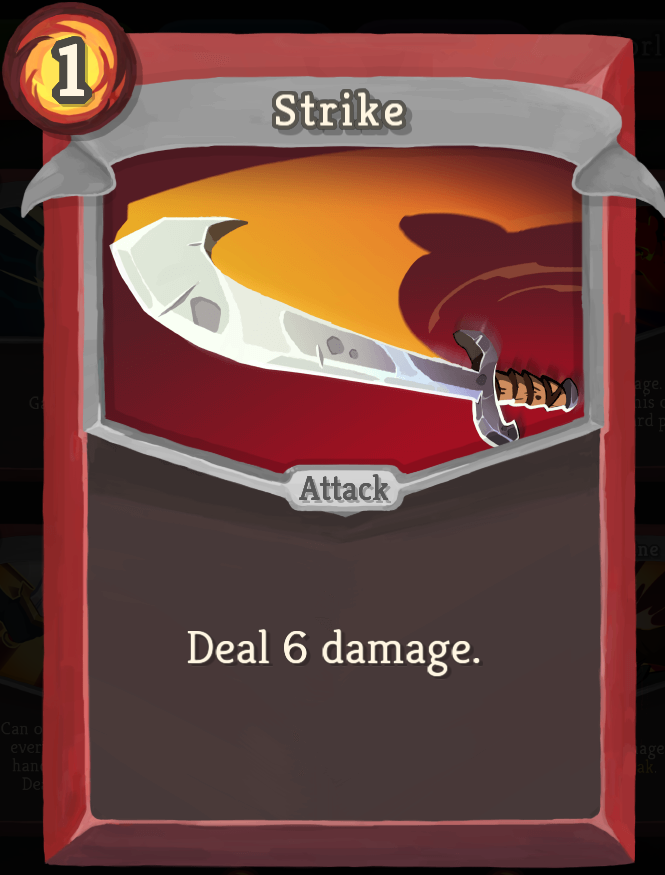
\includegraphics[width=0.95\textwidth]{img/Slay-the-Spire-Strike.png}
        \label{fig:sts-strike}
    \end{minipage}%
    \begin{minipage}{.25\textwidth}
        \centering
        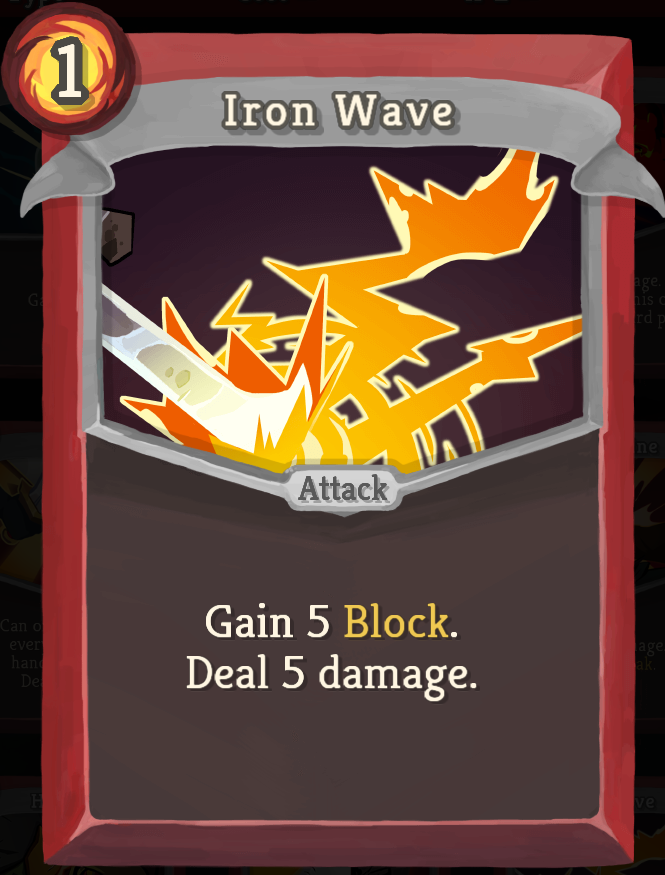
\includegraphics[width=0.95\textwidth]{img/Slay-the-Spire-Iron-Wave.png}
        \label{fig:sts-iron-wave}
    \end{minipage}%
    \begin{minipage}{.25\textwidth}
        \centering
        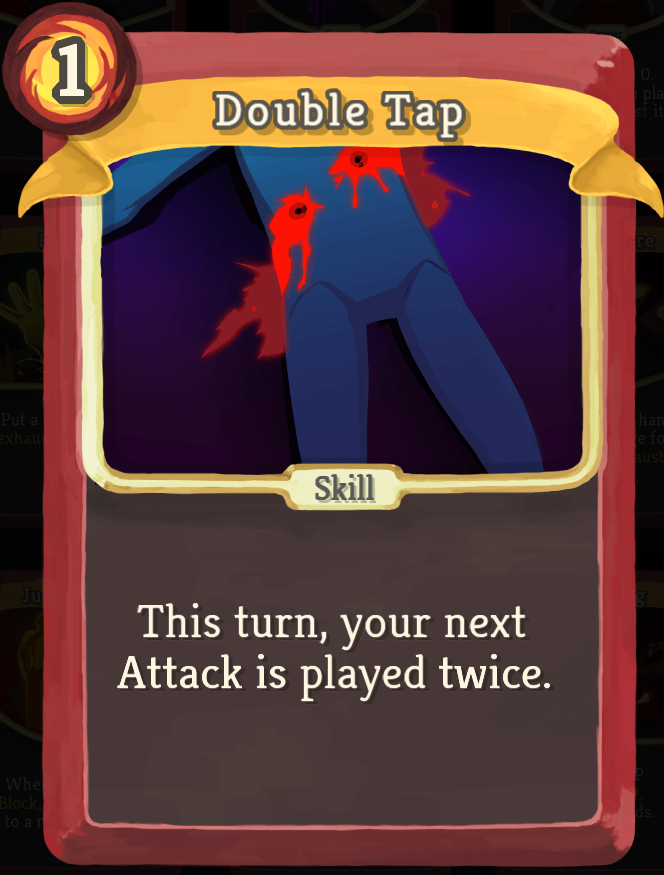
\includegraphics[width=0.95\textwidth]{img/Slay-the-Spire-Double-Tap.png}
        \label{fig:sts-double-tap}
    \end{minipage}
    \caption{\emph{Defend}, \emph{Strike}, \emph{Iron Wave} and \emph{Double Tap}---cards from \emph{Slay the Spire.}}
\end{center}

\?{Should I transcribe the cards}
The player starts each run with several copies of \emph{Defend} and \emph{Strike} in their deck.
Compared to them, \emph{Iron Wave} is very cost-efficient.
It does almost the same thing as \emph{Defend} \textbf{and} \emph{Strike} combined, but for the cost of 1\,\emph{energy}, the same as \emph{Defend} \textbf{or} \emph{Strike}.
Picking this card can help a lot in the early fights, however, it doesn't really grow stronger later in the run.
\emph{Double Tap}, on the other hand, is not great at the start.
In essence, it acts like another \emph{Strike} most of the time, and is useful only when the player draws another attack alongside it.
It is however very strong when your deck contains many attacks that cost a lot of energy but deal much more damage.
Then it allows the player to play a powerful attack twice at the cost of only one more energy.
We can design the blueprints in our game similarly, making some useful early in the run and some powerful later.

\subsection{Make Various Builds Viable} \label{sec:goal-various-builds}

The player should be able to beat the game with a lot of different combinations of blueprints.
We want the player to experiment with different builds, but that will never happen if only few of them are good enough.

- StS --- some cards interact in interesting ways that make them stronger ; there are cards and relics which fundamentally change the way your deck works (ex. barricade and entrench) nerfing some builds is important

\begin{figure}[htb]
    \centering
    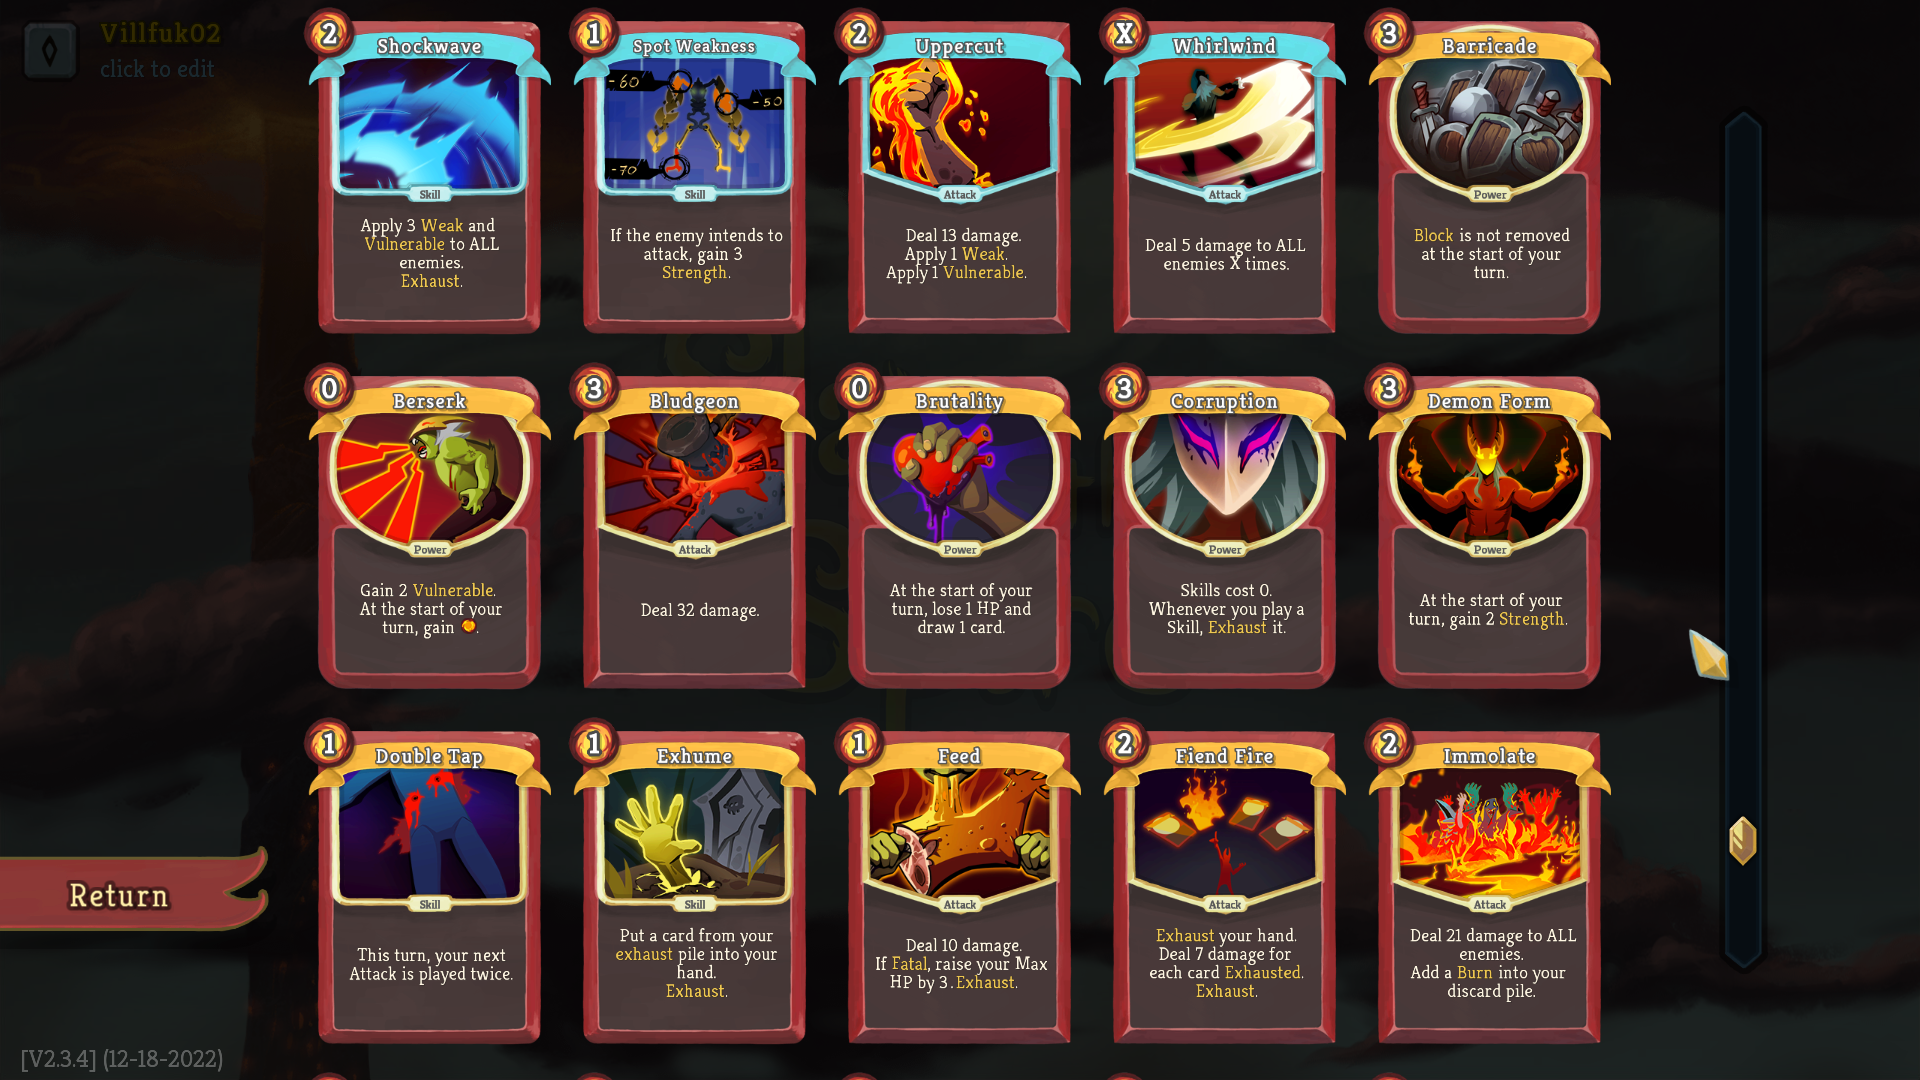
\includegraphics[width=0.8\textwidth]{img/Slay-the-Spire-Compendium.png}
    \caption{A small portion of the many interesting cards in Slay the Spire, viewed in the in-game compendium.}
    \label{fig:slay-the-spire-compendium}
\end{figure}

- PvZ --- the interactions are not so strong, but you have to combine the plants such that you have no weak spots --- cheap and expensive, for specific zombie types

\begin{figure}[htb]
    \centering
    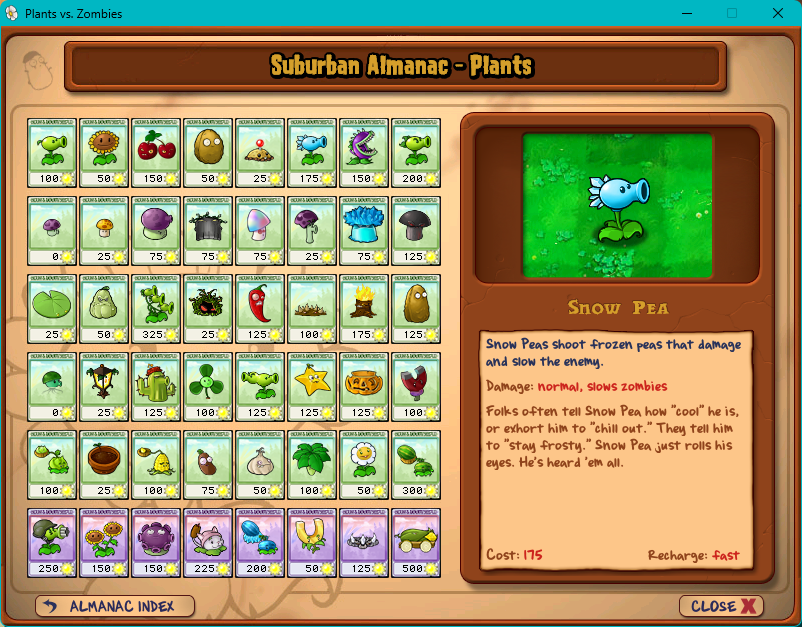
\includegraphics[width=0.8\textwidth]{img/Plants-vs-Zombies-Almanac.png}
    \caption{All the plants of Plants vs.\ Zombies in the in-game almanac.}
    \label{fig:plants-vs-zombies-almanac}
\end{figure}

- make blueprints that have unique effects that change the way you play

\subsection{Force Exploration} \label{sec:goal-force-exploration}

The player will have to use a different build every run.
We don't want the player to just find a single build that works and never explore anything new.
When the player is familiar with a build, it becomes stronger, since they know how to use it effectively.
This discourages them from trying other builds, because they can't use them so well, making them weaker.
Thus, we need to force the player to explore and make them put effort into learning other strategies.

- StS --- you have to explore different strategies because you get different cards every time, some enemies ensure you are prepared for everything and intentionally break some strategies

- characters

\begin{figure}[htb]
    \centering
    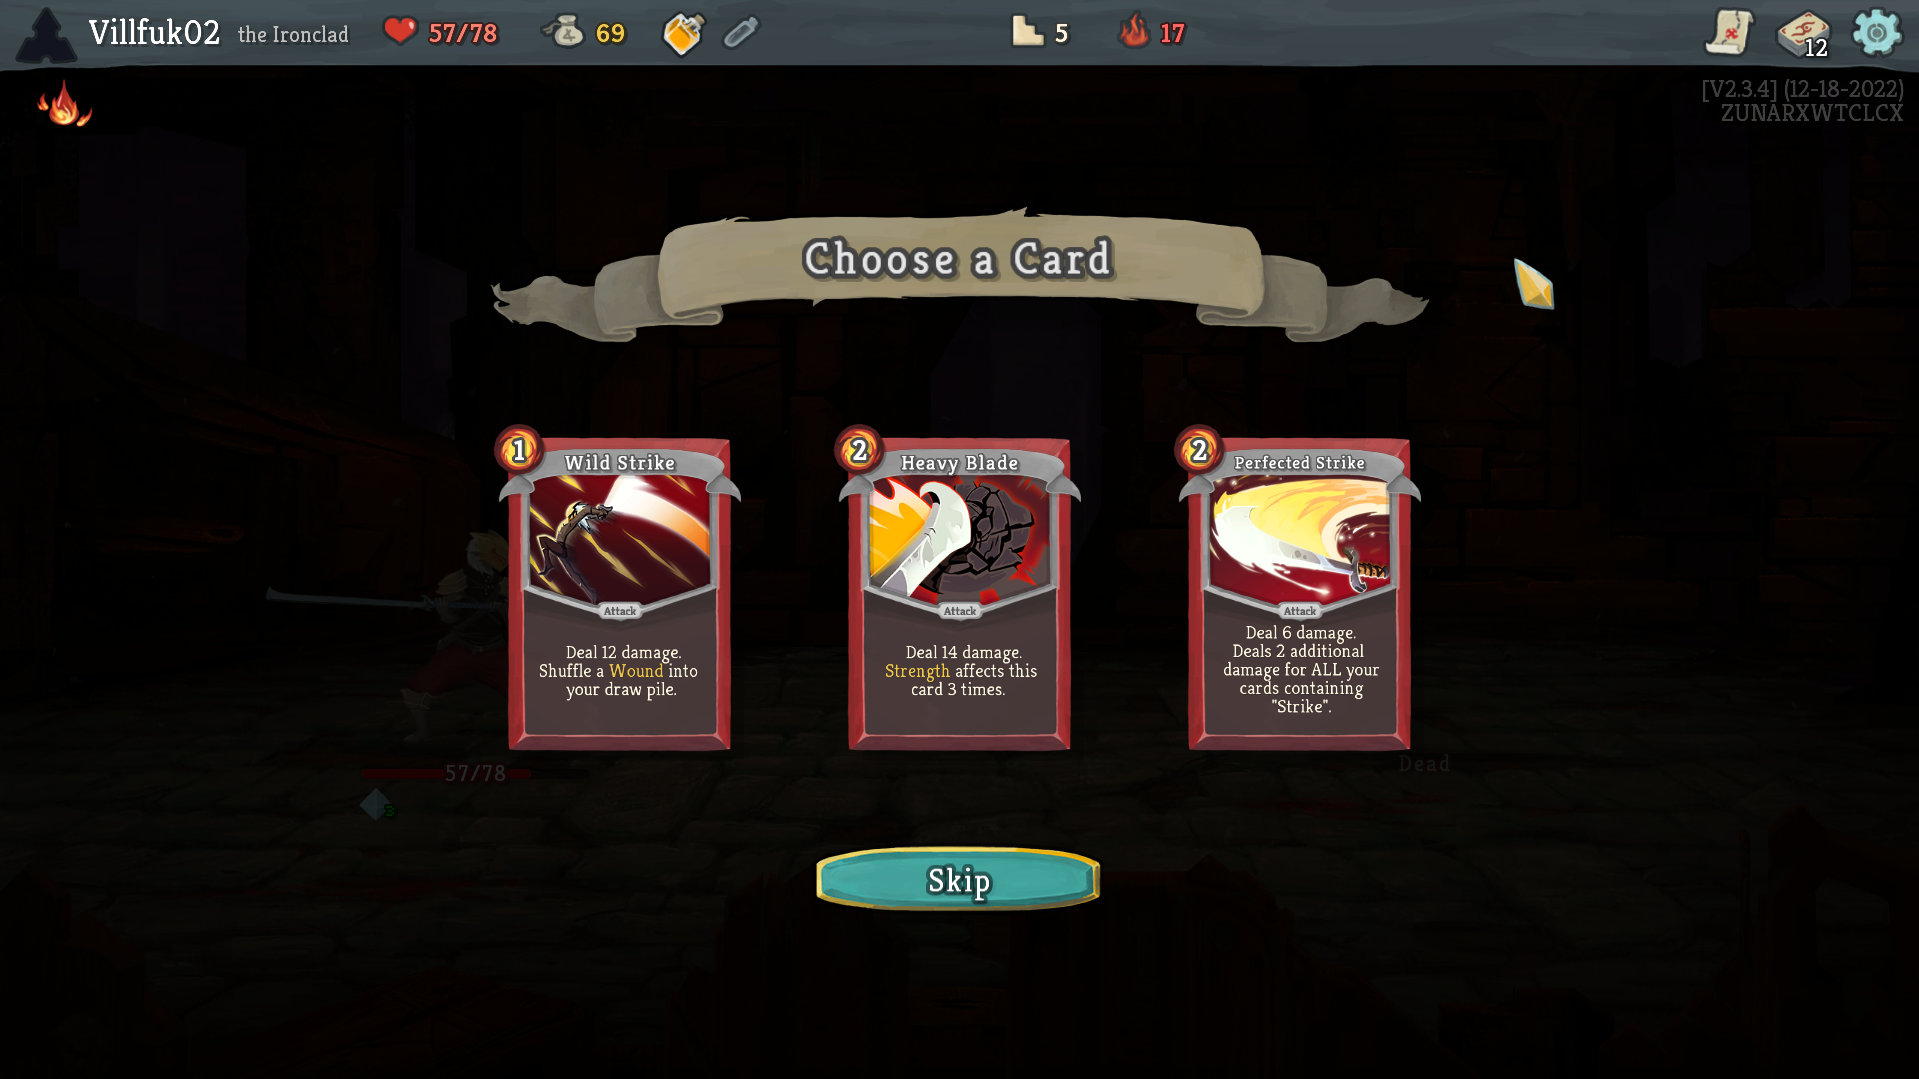
\includegraphics[width=0.8\textwidth]{img/Slay-the-Spire-Reward.png}
    \caption{Card reward screen in Slay the Spire. Here the player can choose on of three randomly selected cards to add to their deck.}
    \label{fig:slay-the-spire-reward}
\end{figure}

- PvZ --- you have to explore different strategies because you have to adapt to different zombies and level environments, not too deep; after the campaign, three seed slots are selected for you.

\begin{figure}[htb]
    \centering
    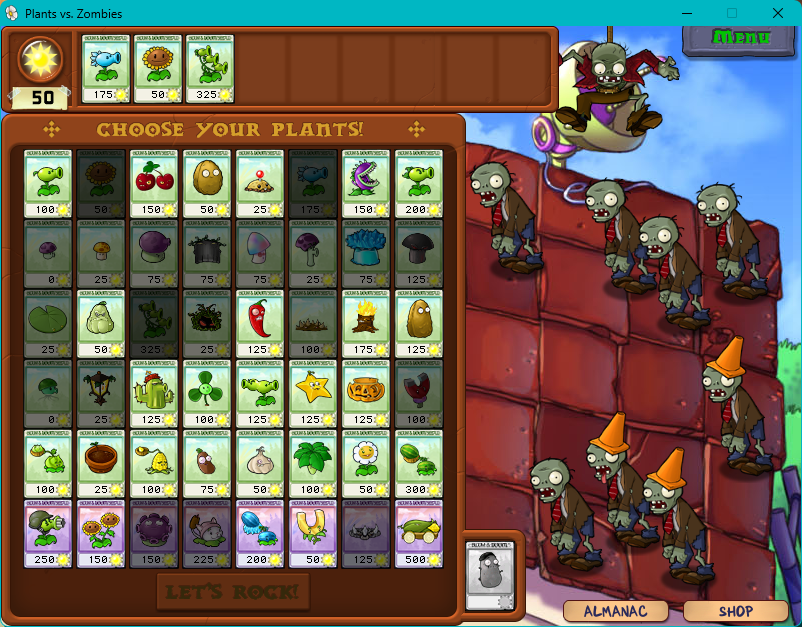
\includegraphics[width=0.8\textwidth]{img/Plants-vs-Zombies-Rooftop.png}
    \caption{Seed select screen in a rooftop level. Here, plants must be planted in flower pots, and most plants cannot shoot uphill.}
    \label{fig:plants-vs-zombies-roof}
\end{figure}

- choose from random blueprints, various attackers with abilities and terrain types

\subsection{Provide a Challenge} \label{sec:goal-challenge}

The player should always have some goal to work towards, just out of their reach.
If the game is too easy, the players will have no reason to think strategically or learn.
Always having a harder challenge to overcome will motivate the player to improve.

- StS --- not easy to beat; after you beat the game, you can play on a higher ascension

\begin{figure}
    \centering
    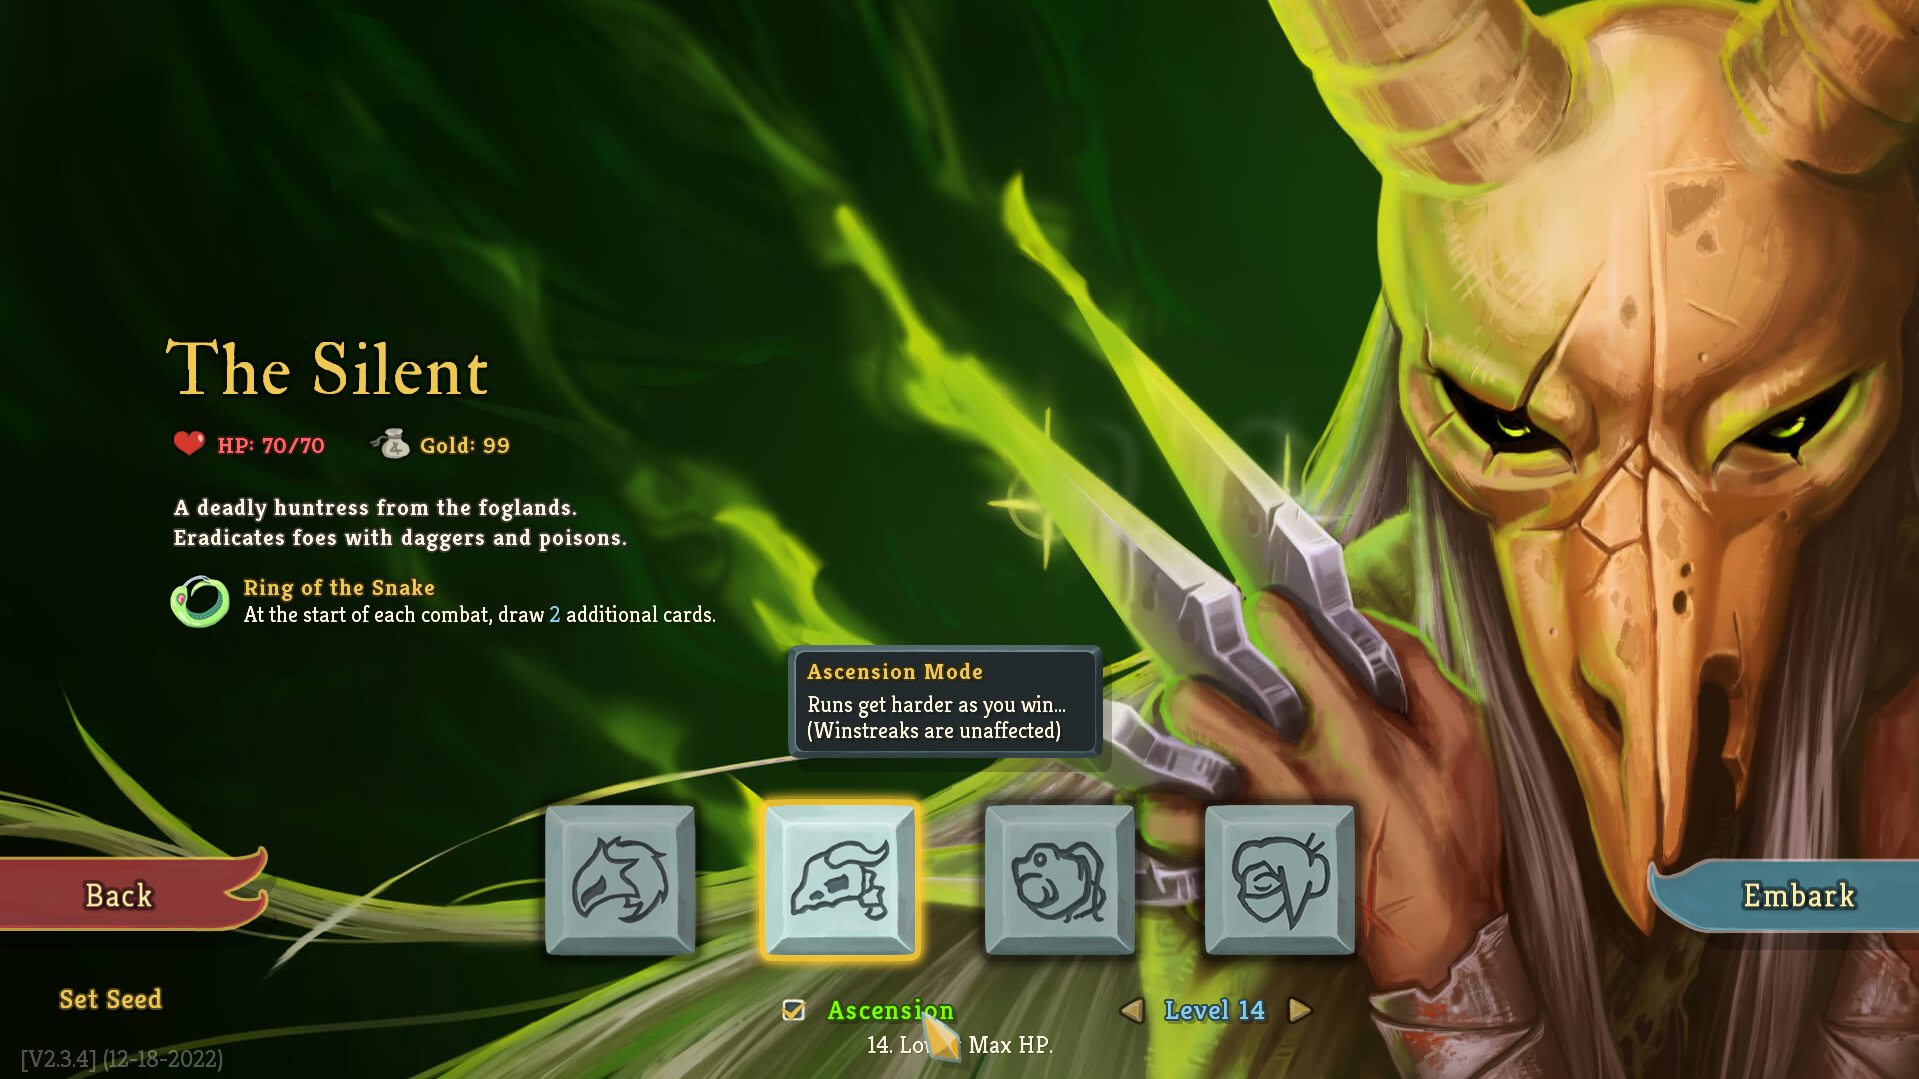
\includegraphics[width=0.8\textwidth]{img/Slay-the-Spire-Ascension.png}
    \caption{Character select screen in Slay the Spire. Here the player can also choose their ascension level, making the game harder.}
    \label{fig:slay-the-spire-ascension}
\end{figure}

- we will have something similar to StS

\section{Battle}

- build stuff, send waves, use abilities

\section{Attacker Movement}

- free movement with individual pathfinding X

- too unpredictable for the player --- The player needs to plan in advance in order to maximize the possibility to take calculated risks
- solution: visualize enemy paths --- Too many different paths - too much clutter; Still planning at most one wave in advance

- linear lanes (like in Plants vs.\ Zombies) X
- not enough space for interesting building placement

- paths based on your buildings X
- what if they block off the path?

- predefined paths \checkmark

- branching

- other qualities

\section{World}

- free placement X

- grid of tiles \checkmark
- more granularity, easier to develop intuition, same for attacker paths

- hexagons X

- squares \checkmark

- 3D \checkmark
- Simple and intuitive way to make the level itself more interesting
Some towers won't be able to shoot uphill or downhill - more interesting decisions for the player

- Terrain types (for now, just one)

- Obstacles

\section{Resources}

\xxx{for each subsection: what is it, why is it, how to acquire it, what are the constraints}

\subsection{Materials}

\subsection{Energy}

\subsection{Hull}

\section{Graphical User Interface}

\xxx{specify controls}

\subsection{Waves Left and Fuel}

\subsection{Hull}

\subsection{Wave Preview}

\subsection{Materials and Energy}

\subsection{Blueprints}

- what they represent

- limited number

- cost and cooldowns

- rarities

- make them unique

- lenticular design

\subsection{Info Panel and Selection}

- what it looks like and what's on it

- select blueprints

- select buildings

- select attackers

\subsection{Highlights and Range Visualization}

\section{Attackers}

- move, have health

- sizes

- special abilities - passive, repeating, reactive

\section{Buildings}

- how and when to build, one per tile

- special building have special abilities

- main types:

\subsection{Economic buildings}

-provide resources

\subsection{Towers}

- attack attackers

- range

- targeting

- projectile types

- damage types

\section{Abilities}

- used mid-wave

- usually instant effects

- free placement, global placement, tile placement, use on a building

\section{Camera controls}

- zoom to look closely, rotate so the terrain doesn't hide stuff

\section{Future Features}

- run structure

- map

- events and shops

- difficulty levels

- unlocks
